\section{Heurística de búsqueda local}
\subsection{Introducción}
Las heurísticas de búsqueda local son capaces de iterar sobre cualquier solución dada y
mejorarla, buscando soluciones vecinas a la solución inicial.

Para plantear la búsqueda local tenemos que definir sobre qué soluciones vecinas buscará el algoritmo. Es decir, tenemos que definir una relación de vecindad entre el espacio de soluciones del problema. Para que el enfoque no sea complejo, definimos 3 vecindades simples:

\begin{enumerate}
	\item Agregar un nodo a la clique, siempre y cuando siga manteniendo la propiedad de clique.

	\item Eliminar un nodo perteneciente a la clique.

	\item Intercambiar un nodo de la clique por uno que no pertenezca a ella.

\end{enumerate}

Ya definidas las vecindades, lo que vamos a hacer en el algoritmo es buscar entre estas soluciones vecinas y quedarnos con la que más nos mejore la frontera, repitiendo este procedimiento hasta que las soluciones encontradas no mejoren.


\subsection{Desarrollo}
Si bien es cierto que la idea de realizar un LocalSearch puede ser aplicada de manera ajena a la solución constructiva golosa que vimos anteriormente, optamos por juntar ambas heurísticas de manera que cada una de las soluciones alternativas que se generen tengan un desarrollo constructivo goloso detrás. De este modo, lo que buscamos es darle a Local la responsabilidad de generar rutas alternativas, con nodos que descartamos en nuestra primera construcción, y a partir de ellas volver a encargarle a nuestro algoritmo constructivo que alcance una solución golosa.

De este modo, si repasamos las vecindades definidas anteriormente, notaremos que tanto agregar como eliminar nodos no son opciones que vayan a servirnos (por lo menos, hasta que apliquemos una nueva heurística sobre estas dos), puesto que Local Search recibirá siempre un algoritmo construido mediante la heurística golosa, donde todos los nodos agregados implican un crecimiento de la frontera y donde no hay ningun nodo externo que agrande la misma.

Por ende, dentro de las vecindades solo nos interesa intercambiar tanto uno como dos nodos de la clique, y a partir de esta nueva clique generar un resultado goloso. No es dificil notar que la vecindad, aún quitándole dos nodos y agregando dos nuevos, es pequeña: para casos con $n$ grande, el hecho de intercambiar solo dos nodos de una solución golosa dificilmente nos lleve a la CMF. Sin embargo, el hecho de correr el algoritmo hasta que no se consigan mejoras puede acercarnos bastante a esta solución, más si consideramos que detrás de la búsqueda local hay una heurística golosa que, para cada iteración, encuentra una solución constructiva aún mejor que la anterior.

Es importante ver que siempre será necesario devolver la solución alternativa luego de aplicarle el algoritmo goloso, puesto que de otro modo podríamos descartar una solución mejor a la actual de manera errónea. Si tomamos nuestra solución inicial, le quitamos dos nodos y le agregamos dos nuevos, si bien es posible que este nuevo grafo tenga una frontera mayor al anterior, también podría ocurrir que se genere una clique de peor solución parcial, pero que al aplicarle el algoritmo goloso nos lleve a una clique con una frontera mayor a la que teníamos. Esto pasaría porque conseguimos armar una clique adyacente a nodos que anteriormente no habíamos considerado, y que finalmente resultaron ser una mejor solución para nuestro problema.

Imaginémoslo con dos montañas, para acercarnos de manera intuitiva. Nosotros estamos parados actualmente en el pico de una montaña, pero al caminar dos pasos para abajo y dos hacia arriba a la derecha, encontramos un camino nuevo. Bien podríamos descartarlo, porque la altura en la que estamos parados actualmente es menor que la anterior, pero al subirlo podríamos acabar en un pico más alto que el anterior. Es por esto que, a la hora de obtener la solución, es mejor tener en cuenta cuál es el pico más alto que puede alcanzar la nueva clique.

Por lo tanto, acabaremos encontrando o bien nuevas soluciones, o bien la misma solución que encontramos en el algoritmo goloso inicial, de forma que siempre acabaremos teniendo un resultado mejor o igual al que se conseguía con la heurística constructiva aislada.

Teniendo esto en cuenta, quedarían definidas de la siguiente manera las vecindades y el resultado obtenido de cada una de ellas. Como las búsquedas de cada tipo de vecindad son diferentes entre sí, vamos a implementar una función que nos encuentre la mejor solución para cada tipo y después vamos a comparar estas soluciones. Esto nos trae el beneficio de que, en caso de agregar nuevas vecindades, no deberemos tocar mucho la implementación.

\subsubsection{Vecindad: Agregar Nodo}

Esta vecindad es la que se aplica en la heurística golosa constructiva. Como ya vimos, la solución que nos va a mejorar más la frontera será agregar el nodo que mantenga la clique y tenga mayor grado.

\begin{algorithm}[H]
	\NoCaptionOfAlgo
	\caption{\algoritmo{localAgregar}{\In{listaAdyacencia}{lista}, \Inout{clique}{solucion}}{}}

    nodosAdyacentes $\leftarrow$ adyacentes(lista, mayor)

    ordenarPorGrado(nodosAdyacentes)

    \For{$i \leftarrow 0$ \KwTo nodosAdyacentes.largo}{
		\If{esAdyacenteATodos(nodosAdyacentes[i], solucion, listaAdyacencia) $\land$ \\ aumentaLaFrontera(nodosAdyacentes[i], solucion, listaAdyacencia)}{
			agregarNodoAClique(solucion, nodosAdyacentes[i])

			break
	    }
    }
    
    solucion $\leftarrow$ algoritmoGoloso(solucion, listaAdyacencia)
\end{algorithm}

\subsubsection{Vecindad: Eliminar Nodo}

Aquí queremos encontrar nodos que al eliminarlos nos aumenten la frontera. Estos nodos van a tener la característica de tener más adyacentes en la clique que afuera, ya que si por ejemplo el nodo $j$ perteneciente a la clique tiene 2 adyacencias por afuera de la misma y esta es de grado 4(por lo que tendrá 3 adyacentes pertenecientes a la clique) al eliminarlo, la frontera perderá los 2 ejes adyacentes a $j$, pero ganará los 3 ejes que llegan de la clique a $j$. Por lo tanto, podemos definir el beneficio de eliminar un nodo de la clique como $2 * (grado de la clique - 1) - cantidad de adyacentes al nodo$.

La implementación es bastante directa, recorremos los nodos de la clique y buscamos el que más nos aporte a la frontera si lo eliminamos.

\begin{algorithm}[H]
	\NoCaptionOfAlgo
	\caption{\algoritmo{localEliminar}{\In{listaAdyacencia}{lista}, \Inout{clique}{solucion}}{}}

    mejora $\leftarrow$ 0

    \For{$i \leftarrow 0$ \KwTo solucion.nodos.largo}{
        mejoraNodo $\leftarrow$ (solucion.nodos.largo - 1) - adyacentesA(lista, solucion.nodos[i]).largo

		\If{mejoraNodo $>$ mejora)}{
			nodoABorrar $\leftarrow$ i

			mejora $\leftarrow$ mejoraNodo
	    }
    }

    \If{mejora $>$ 0)}{
        borrarNodoClique(solucion, solucion.nodos[nodoABorrar])
    }
    
    solucion $\leftarrow$ algoritmoGoloso(solucion, listaAdyacencia)

\end{algorithm}

\subsubsection{Vecindad: Intercambiar Nodo}

Para encontrar el par de nodos(uno interno a la clique y otro externo) que mejoren la clique, lo que vamos a hacer es recorrer los nodos internos y, por cada nodo, buscar en los ejes externos cuanto nos mejora la solución si los intercambiamos.

\begin{algorithm}[H]
	\NoCaptionOfAlgo
	\caption{\algoritmo{localIntercambiar}{\In{listaAdyacencia}{lista}, \Inout{clique}{solucion}}{}}

    mejora $\leftarrow$ 0

    \For{$i \leftarrow 0$ \KwTo solucion.nodos.largo}{
        \For{$j \leftarrow 0$ \KwTo solucion.nodosExternos.largo}{

            mejoraNodo $\leftarrow$ mejoraEnFronteraAlIntercambiar(solucion.nodosExternos[j], solucion.nodos[i], solucion, listaAdyacencia)

            \If{esAdyacenteATodosMenosA(solucion.nodosExternos[j], solucion.nodos[i], solucion, listaAdyacencia) $\land$ \\ mejoraNodo $>$ mejora }{
                nodoABorrar $\leftarrow$ i

                nodoAAgregar $\leftarrow$ j

                mejora $\leftarrow$ mejoraNodo
            }

        }
    }

    \If{mejora $>$ 0)}{
        borrarNodoClique(solucion, nodoABorrar[nodoABorrar])

        agregarNodoClique(solucion, solucion.nodos[nodoAAgregar])
    }
    
    solucion $\leftarrow$ algoritmoGoloso(solucion, listaAdyacencia)

\end{algorithm}

\subsubsection{Algoritmo final}
Finalmente, considerando estas cuatro vecindades, acabaremos teniendo un algoritmo general de este estilo:

\begin{algorithm}[H]
 \NoCaptionOfAlgo
 \caption{\algoritmo{heuristicaDeBusquedaLocal}{\In{listaAdyacencia}{lista}, \Inout{clique}{solucion}}{}}

    \While {esMejor}{
        esMejor $\leftarrow$ falso

        posibleMejorSolucion $\leftarrow$ buscarMejorSolucionVecina(lista, solucion)

        \If{posibleMejorSolucion.frontera $>$ solucion.frontera)}{
            esMejor $\leftarrow$ verdadero

            solucion $\leftarrow$ posibleMejorSolucion
        }
    }

\end{algorithm}

Donde buscarMejorSolucionVecina corre las tres vecindades y se fija cual es la mejor.

\subsection{Complejidad Temporal}
Para analizar la complejidad temporal de este ejercicio, debemos analizar la complejidad de cada una de los algoritmos que corremos para realizar la búsqueda en sus vecindades. Por lo tanto, tendremos las siguientes complejidades:

\begin{center}
	\textbf{Agregar nodo}
\end{center}
Este algoritmo recorre las adyacencias de uno de los nodos de la clique (cualquiera, por lo que recorre como máximo $|maxAdyacente|$ nodos) y, para cada uno de ellos, chequea si es o no adyacente a los nodos de la clique, y si agregarlo aumenta la frontera. Por lo tanto, con cada nodo se fijará si el vértice es adyacente a la clique y realizará el cálculo correspondiente. Como vimos anteriormente, el algoritmo \textbf{esAdyacenteATodos} tiene una cota temporal de $O(n)$, mientras que el cálculo correspondiente a la frontera se realiza en $O(1)$. Por ende, acabamos teniendo $|maxAdyacente|$ veces que realizar una operación de complejidad $O(n)$, y como vimos en el análisis de la heurística golosa que $O(|maxAdyacente|)$ $\subseteq$ $O(min(n,m))$, acabamos teniendo $O(min(n,m)$ $\times$ $n)$. A esta solución obtenida le aplicamos finalmente el \textbf{Algoritmo Goloso}, cuya complejidad vimos que es $O(min(n,m)$ $\times$ $n)$, por lo que acabaríamos teniendo $O(2 (min(n,m)$ $\times$ $n))$, que termina siendo $O(min(n,m)$ $\times$ $n)$.

\begin{center}
	\textbf{Eliminar nodo}
\end{center}
Este algoritmo recorre los nodos de la clique (como máximo, $min(n,m)$ nodos) y para cada uno de ellos se fija si, al quitar este nodo, la frontera de la clique mejora. Como nuevamente, lo único que tenemos que hacer es realizar el cálculo de la frontera en $O(1)$, la complejidad de este ciclo será $O(min(n,m))$. Finalmente, como vimos, le corremos el \textbf{Algoritmo Goloso} a la solución, lo cual tiene una complejidad $O(min(n,m)$ $\times$ $n)$. Por ende, acotamos y definimos que la cota temporal de Eliminar Nodo es $O(min(n,m)$ $\times$ $n)$.

\begin{center}
	\textbf{Intercambiar nodos}
\end{center}
Este algoritmo, básicamente, consta de dos ciclos: el primero, que recorre cada uno de los nodos de la clique (a través de la variable $i$); y el segundo, que recorre la lista de adyacencia de uno de los nodos de la clique (particularmente, el del nodo $i+1$). Por lo tanto, tenemos:

\textbf{Para cada nodo $i$ en la clique, para cada nodo $j$ adyacente a $i+1$, agregar $j$ y sacar $i$}

Esto significa que tenemos dos ciclos que dependen del tamaño de la clique y, por ende, del mayor grado de la clique (es decir, $|maxAdyacente|$). Por lo tanto, al tener dos ciclos anidados, acabamos teniendo $O(|maxAdyacente|$ $\times$ $|maxAdyacente|)$, que acotamos por $O((min(n,m))^2)$. 

Ahora, queda ver que es lo que ocurre adentro del ciclo. Luego de quitar el nodo $i$, debemos fijarnos si el nodo $j$ es adyacente a todos los que quedaron en la clique. Para esto, utilizamos \textbf{esAdyacenteATodos}, que tiene una complejidad de $O(n)$, y en caso de que efectivamente sea adyacente, agregamos el nodo $j$ a la clique y le corremos el \textbf{Algoritmo Goloso}, para luego comparar si el resultado obtenido es mejor. Esto quiere decir que, para cada iteración, corremos $O(n + min(n,m)$ $\times$ $n)$. Por ende, al acotar este algoritmo, tendremos un ciclo de $min(n,m)^2$ pasos de complejidad $O(min(n,m)$ $\times$ $n)$. Es decir, y finalizando con la cota de \textbf{Intercambiar Nodos}, que la complejidad es de $O((min(n,m))^3$ $\times$ $n)$

\bigskip

Así, alcanzamos las complejidades de cada una de nuestras vecindades. Por lo tanto, la complejidad de buscar la mejor solución vecina será $O(min(n,m)$ $\times$ $n + min(n,m)$ $\times$ $n + (min(n,m))^3$ $\times$ $n)$, que por propiedades de O grande se acota finalmente con $O((min(n,m))^3$ $\times$ $n)$. Puesto que el algoritmo general es, simplemente, tomar una clique y correrle el algoritmo hasta que no mejore, el mismo correrá un máximo de $n$ veces (puede agregar o sacar cada nodo una vez, y no tiene sentido que lo haga más veces, ya que esto implicaría contradecir decisiones anteriores que mejoraban la solución). Por lo tanto, al considerar el peor caso, habremos corrido $n$ veces un algoritmo de costo $O((min(n,m))^3$ $\times$ $n)$, dejándonos con una complejidad temporal final de $O((min(n,m))^3$ $\times$ $n^2)$

\subsection{Casos Patológicos}

Los casos patológicos de la heurística de búsqueda local tienen la complejidad de que partimos de una solución, por lo que si la solución original no es vecina a la mejor solución no vamos a poder encontrarla. Podemos afirmar que la familia de instancias que definimos en la heurística golosa, tambien son malos casos para esta heurística, ya que la solución que nos entrega la golosa, no se encuentra en la vecindad de la la solución óptima, por lo que no lograremos alcanzar esta solución. Hay que tener en cuenta que la heurística depende de la solución inicial, por lo que el caso patológico solamente se va a dar si la solución inicial es la que estamos describiendo.

\subsection{Experimentación}

Al igual que con la heurística golosa, el tiempo de ejecución de este algoritmo depende de varios aspectos del grafo, además de $n$ y $m$. Por esto, decidimos solo realizar un análisis del peor caso para comprobar las cotas propestas.

\noindent
\begin{minipage}{0.55\textwidth}
    \hfill
    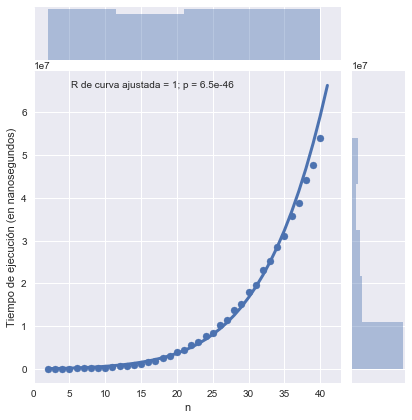
\includegraphics[scale=0.6]{img/local-n.png}
\end{minipage}
\hfill
\begin{minipage}{0.44\textwidth}
    \begin{center}
        Datos del gráfico

        \begin{tabular}{ | l l |}
            \hline
            Grafo completo & $m = \frac{n * (n-1)}{2}$\\ 
            Curva aproximada & $f(x) = (x^5) / 2 + 5000 * x^2$ \\
            \hline
        \end{tabular}
    \end{center}
\end{minipage}

Dado que el exponente que forma parte de nuestra cota de complejidad es bastante elevado, decidimos observar estos mismos datos con 2 enfoques distintos: por un lado, en escala logarítimica, y por el otro, en base a m (que, al ser grafos completos, equivale a $n^2$).


\noindent
\begin{minipage}{0.55\textwidth}
    \hfill
    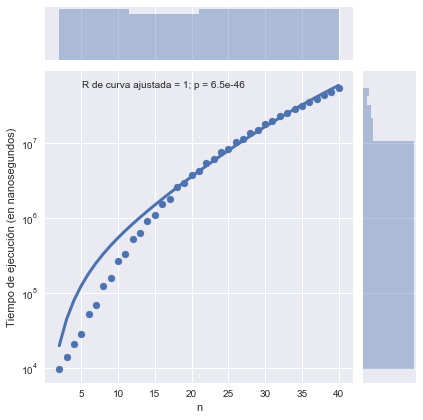
\includegraphics[scale=0.6]{img/local-n-log.png}
\end{minipage}
\hfill
\begin{minipage}{0.44\textwidth}
    \begin{center}
        Datos del gráfico

        \begin{tabular}{ | l l |}
            \hline
            Grafo completo & $m = \frac{n * (n-1)}{2}$\\ 
            Curva aproximada & $f(x) = (x^5) / 2 + 5000 * x^2$ \\
            \hline
        \end{tabular}
    \end{center}
\end{minipage}

\noindent
\begin{minipage}{0.55\textwidth}
    \hfill
    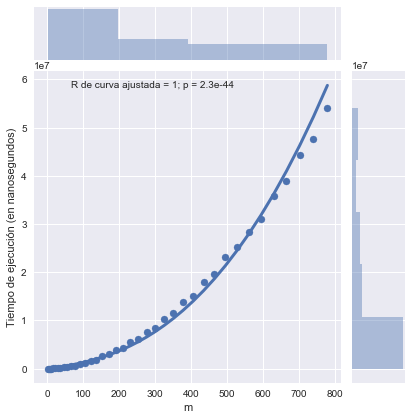
\includegraphics[scale=0.6]{img/local-m.png}
\end{minipage}
\hfill
\begin{minipage}{0.44\textwidth}
    \begin{center}
        Datos del gráfico

        \begin{tabular}{ | l l |}
            \hline
            Grafo completo & $m = \frac{n * (n-1)}{2}$\\ 
            Curva aproximada & $f(x) = 3 * (x^{2.5}) + 10000 * x$ \\
            \hline
        \end{tabular}
    \end{center}
\end{minipage}

Podemos notar en estos gráficos que las constantes elegidas para las curvas están un poco sobreajustadas. Sin embargo, utilizando el R de Pearson podemos aseverar que la complejidad en sí es correcta, ya que este coeficiente detecta correlaciones lineales y no depende de las constantes asociadas a cada elemento.